\thesischapter{Background: Traditional Railway Control Systems}{Background: Traditional Railway Control Systems}
\chaptermark{Traditional Railway Control Systems}

The birth of the railways occurred in the 1800s and from that point until the present day they have experienced continual growth, change and development. In the beginning the burden of safety was placed solely on human shoulders and has since been placed on mechanical systems before finally being transferred to electronics systems that are in place guaranteeing safety today. In the following we shall present a brief history of the railway followed by information on our industrial partner Invensys Rail.  Following this general introduction we shall look into specific equipment found on the modern railway and other information needed to understand the domain. Most importantly we shall describe the Westrace interlocking, a modern system charged with guaranteeing safety on the railway, which is produced by Invensys. In the final part of this chapter we shall look at some previous work in this field.


\begin{comment}
From their birth in the 1800s to the present day, the railway and its control
systems have seen many advances. Its control and safety has gone from being a
completely manual human based system, to a mechanical system and finally to the electronic
system we see today. We will now look at a brief history of the railway
followed by information on our industrial partner Invensys Rail. We then look
more closely at modern railways and the equipment which constitutes
them. We also study
Westrace interlocking which is produced by Invensys and the
ladder logic programs which run on it. Finally, we look at some previous work
in this field.
\end{comment}

\section{ A History of Railway Signalling and Control Systems}
Initially in the early days of the railway there was not fixed signals as we see today. Instead Policemen, stationed at junctions and railway stations, were charged with signalling train drivers using a system of flags or oil lamps and changing the points\footnote{A point is a physical device that joins two seperate tracks and controls the flow of trains in one direction or the other} of the railway. A major problem of the time, without telecommunications, was that there was no way of locating a train once it went out of sight. This meant that in practice the only safety precaution that could be taken was to delay the departure of trains using an egg timer which would hopefully space out their positions along the track. The level of safety resulting from this precaution was acceptable as train speeds were not relatively high at the time compared with modern railways.


\begin{comment}
Prior to the days of fixed signals, Policemen would be stationed at
junctions and railway stations. They changed points manually and gave instructions to train drivers
by using a system of either flags or oil lamps depending on the
visibility. Since this was before the time of telecommunications and
electricity there was no way of telling where a train was once it left a
station and went out of sight. The only safety precaution that could be taken
was to use an egg timer to delay the departure of the next train in order to
give the previous train time to progress along the track. Train speeds were
not very high during this period so this was an acceptable way of ensuring safety.
\end{comment}


The most important type of signal found in the modern railway is the \emph{fixed signal} which is static, positioned by the side of the track and visually presents information to the train driver. The first fixed signals were wooden boards shaped in such a way as to provide specific information which were attached to poles and rotate around a vertical axis. Typically these boards would form a signal instructing the train driver to stop; however if the board was rotated side-on to the driver then it becomes inactive and the driver would proceed if it was safe to do so.

\begin{comment}
Modern railway signally makes use of \textbf{fixed signals}. These are permanently positioned
by the side of the track and provide some visual information to the train driver.
The original fixed signal consisted of a shaped wooden board that could be
rotated on pole round a vertical axis. If the board was visible to the driver
then he would have to stop the train. On the other hand if the driver couldn't
see the board because it was side-on to him then he would be able to
proceed.
\end{comment}

The next major enhancement of these signals came in the form of the \emph{semaphore} fixed signal.  Instead of having two positions (visible/ not visible), the boards of a semaphore signal could be moved into one of several predetermined positions. The most common of these signals had three visible positions or aspects in which they could be placed which would relay the following information to an approaching driver: proceed if it's safe, proceed with caution if it's safe and stop.

\begin{comment}
One of the major developments in railway signalling was the introduction of
the \textbf{Semaphore} fixed signal. These consisted of a board that could be
moved into several preset positions. Typically these would have  3 different visible
``aspects'' which they could be set to: One aspect to indicate the driver can
proceed, another that indicates the driver can proceed with caution and
finally an aspect which indicates that the driver should stop. 
\end{comment}

The introduction of the semaphore signal also foreshadowed another major change in the system for controlling the signals behind the scenes.  A new band of professional \emph{signallers} were employed to specifically manage the railways, replacing the policemen that proceeded them in the progress. The efficiency of signal control was also improved by a system of wires, pulleys and levers which enabled multiple signals and points to be controlled from a central position. This central position was typically enclosed in a box -- giving rise to the name \emph{signal box} -- which was typically manned by one or more signallers. The controlling signals and points from the centrality of the signal box also enabled for more safety mechanisms to be installed. The most prominent of these -- the \emph{interlocking}  -- shall be the subject of interest to us in later chapters. The interlocking physically prevented the control system of a railway from entering an unsafe state by physically locking levers.


\begin{comment}
Around about the same time as the introduction of the semaphore signal, the system
for controlling the signals went under drastic change. The Policemen were
replaced with professional \textbf{Signallers} whose job was specifically to
manage the railways. A system of pulleys, wires and levers was also devised
to allow multiple signals and points to be controlled from a central
position. This central position became known as a \textbf{signal box} and was
manned by one or more signallers. This centralisation allowed for further
safety mechanisms to be installed. One in particular, namely the \textbf{interlocking},
is of interest to us. The interlocking physically locked levers if they were
unsafe to move.
\end{comment}
The advent of electricity brought about a further advance in railway technology, allowing for the development of the \textbf{track circuit}. When a train was on a segment of track it completed the circuit between the two rails and lit up an indicator in the signal box. As more track circuits were deployed it became possible to control certain signals without human intervention. These \textbf{automatic signals} were completely operated by track circuits and prevented trains from entering a segment of track behind a signal already containing a train. Electric motors enabled the construction of electric point machines enabling the signaller to electronically control a point at a great distance with little physical effort. The area controlled by each signal box was greatly increased along with the number of signals controllable by one signaller. Electromechanical \textbf{relays} were introduced as a replacement for the solely mechanical relays reducing the size of each signal box and its footprint on the landscape.
\begin{comment}
The next leap in railway technology came from the invention of the electronic
\textbf{track circuit}. These would activate an indicator in the signal box if a
segment of track was occupied by a train. As more and more track circuits
became installed it was no longer necessary to have human intervention to
control certain signals. \textbf{Automatic signals} were introduced which
operated completely by track circuits without any intervention from human
signallers. Around this time \textbf{electric point machines} were introduced
removing a large amount of physical work performed by signallers allowing for
a greater area of control for each signaller.  Around this time
electromechanical \textbf{relays} began to replace purely mechanical relays
reducing the amount of space needed for a signal box.
\end{comment}

Further instances of an electrical system replacing a mechanical one occurred in the 1920s and subsequently in the 1930s. New \textbf{colour light signals} replaced  the mechanical semaphore signals and had the advantage of being brighter than the oil lamps of that signal.
Electronic \textbf{control panels}, which contained switches and buttons, replaced the mechanical levers and removed the remaining physical effort needed to operate signalling systems. The combination of track circuits, electronic points and control panels enabled the introduction of \textbf{route setting} whereby at the press of a single button a configuration of signals and points could be selected thus enabling a train to travel down a particular route along the track.

The next major advancement came some 50 years later and was enabled by the development of microprocessors. The relays and mechanical interlockings were replaced with \textbf{solid state interlockings} which were smaller still and more reliable than relay interlockings.
These solid state interlockings are one of the systems verified later on in chapter \ref{chapter:dpllapp}. Jump forward another 30 years to the current day and we are seeing the development and deployment of a new type of control system which makes use of recent technologies such as GPS and GMS radio  communications that enable signallers to have a far finer grain of control when compared with the discrete track circuits and do not need the physical coloured light signals to function. One such instance of a control system is the European Rail Traffic Management System which is discussed in more detail in Chapter \ref{chapter:ERTMS}
\begin{comment}
In the 1920s \textbf{colour light signals} replaced mechanical semaphore signals these where much brighter than the oil
lamps fitted to semaphores and greatly increased the safety of night time
train travel. In the 1930s the mechanical levers were replaced with an electronic \textbf{control panel}
containing switches and buttons. This allowed for the introduction of
\textbf{route setting} where with the press of a button configurations of signals and points would be
associated with a particular route could become activated. Prior to this time
many levers would have had to have been pulled to set many different pieces of equipment.
During the 1980s the most important advance from our point of view took
place. The advent of electronic microprocessors enabled the replacement of the
relay and mechanical interlockings with an electronic \textbf{solid state interlocking}
system (SSI) \cite{AC08}. The main focus of this project will be to investigate the safety
of such solid state interlockings.
\end{comment}
\section{Invensys Rail}

Siemens Rail Automation \cite{Siemens} has been producing train control equipment and safety devices for over 140 years starting with its original incarnation Westinghouse Rail Systems Ltd and subsequent incarnation Invensys Rail. 
The first such safety device was train air brakes; if the power was cut from the train then the brake would automatically kick in, entering a failsafe state. The company was also charged with supporting British Rail in its development of the first solid state digital railway interlocking to be installed in Leamington Spa. Currently their operations are focused on supplying railway control systems globally with customers in Australia, Hong Kong, Germany , Spain and the UK. One of the products produced by Invensys that we are interesting in is  a solid state interlocking called the Westrace. This interlocking continually receives input from the railway, decides whether or not a request or railway state is safe using a \emph{ladder logic} program and prevents the railway from entering unsafe states. This ladder logic will be explained later in this chapter. Further information on the railway domain including terminology and methodology can be found in a book by David Kerr and Tony Rowbotham (See \cite{KR01}.)
\begin{comment}

Originally they produced air brakes for trains, these had a
failsafe state such that if the power was cut the brakes would automatically stop the train.
Later on in the company's development they provided support to British Rail
when the first solid state digital railway interlocking was installed in
Leamington Spa. Today they supply railway control equipment to companies based
around the globe, including companies based in Australia, Hong Kong,
Germany, Spain and the UK. This project is mainly concerned with one of the
solid state railway interlockings Invensys produces called the Westrace. The
Westrace railway interlocking continuously runs a ladder logic program which
prevents the railway control systems from entering a dangerous state. Ladder
logic will be explained in a later chapter.
David Kerr and Tony Rowbotham  produced a book that explains the
terminology and methodology used in the railway industry and by
Invensys (See \cite{KR01}).  
\end{comment}
\section{An Overview of the Railway Domain} 
In this section we present the features of the railway domain that are in
the scope of this thesis. We hope to provide the reader with the background
information and terminology necessary to understand later chapters.


\subsection{The Railway Topology: Track and Points}
In order to get a better understanding of the railway we will now present a small example physical railway in the form of a junction with a single point. This is a common way of drawing track plans and allows for the topology of a segment of track to be expressed on paper. Further examples and details of the railway topology can be found in \cite{KR01}.


\begin{comment}
We will now present an overview of the physical railway from a topological
point of view. To do this we will present an example of a small track plan
of a junction.  If the reader is interested in learning more about the
topology of the railway a more detailed description can be found in \cite{KR01} 
\end{comment}

\begin{figure}

\begin{center}

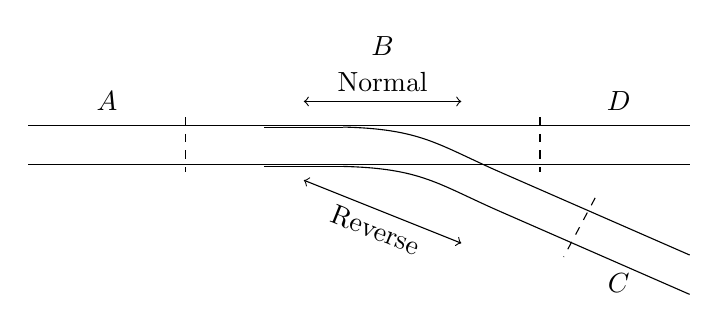
\begin{tikzpicture}

\node at (-4 , 1.3)  {$A$};

\node at (-0.5 , 2) {$B$};

\node at (2.5 , -1) {$C$};

\node at (2.5 , 1.3) {$D$};


\draw[<->] (-1.5, 1.3) to node [above, sloped] {Normal} (0.5 , 1.3) ;

\draw[<->] (-1.5 , 0.3) to  node [below, sloped] {Reverse} (0.5, -0.5);


\draw (-5, 1) -- (3.4,1);




\draw [dashed] (-3 , 1.1)  -- (-3, 0.4);

\draw [dashed] (1.5 , 1.1) -- (1.5 , 0.4);

\draw [dashed] (2.2 , 0.075) -- (1.8, -0.675) ;

\draw (-2, 0.975) -- (-1, 0.975);

\draw (-1, 0.975) .. controls (0, 0.95) and (0.2 , 0.75)  .. (1, 0.4);

\draw (1, 0.4) -- (3.4, -0.65);



\draw (-5, 0.5) -- (3.4, 0.5);

\draw( -2, 0.475) -- (-1, 0.475);

\draw (-1, 0.475) .. controls (0, 0.45) and (0.2 , 0.25)  .. (1, -0.1);

\draw (1, -0.1) -- (3.4, -1.15);





\end{tikzpicture}

\end{center}
\caption{A Typical Junction}

\label{fig:track}

\end{figure}


\subsubsection{Track Segments}

In fig \ref{fig:track}  there are 4 track segments $A,B,C,D$ which is typical of a junction containing a single point. Each track segment contains a track circuit for the purpose of detecting whether it is occupied by a train or not. When a train is present on a segment of track the metal wheels and axle complete the circuit and allow the control system to detect its presence. It is possible for a train to be longer than a track segment and this is particularly the case at junctions and other areas where a large amount of control is needed over trains. A shorter track segment allows for a finer grain view of the railway by the interlocking and control system and can allow for a greater throughput of trains. Conversely the length of track segments can be far longer on long straight segments of track without any interesting features such as junctions or stations.

\begin{comment}
A section of track is typically broken down into track segments each
containing one or more track circuits to detect the presence of a
train. Typically track segments become larger on long straight stretches of
track without any interesting topological features such as junctions or
stations. Likewise track segments become smaller around junctions and stations
where control over train movement is of greater importance. 
\end{comment}


\subsubsection{Points}
Junctions are formed between two tracks using  pieces of equipment called points. The wheels of the train rest on track which makes it physically impossible to just join one track to another as the train would derail.  What is needed is a device that can switch a train off of the track and the point fulfils that role.  Each point can be in one of two positions depending on whether it is actively switching trains off the track which is referred to as \textbf{reverse}  or is inactive which is referred to as \textbf{normal}. The point is one of the main areas of possible danger on the railway. If a train hits the point when it is in the wrong position i.e. from the direction of track segment $B$ to $C$ in fig \ref{fig:track} then the train will derail. There is also a serious danger posed by point moving while a train is on the junction which would also cause a derailment.

\begin{comment}
A point is a physical piece of equipment that is used to 
form a junction. Due to the nature of the rails and trains it is not possible to physically
to just join two segments of track. Instead a point is needed to act as
physical switch controlling the flow of trains through a junction. A point
has two positions which are referred to as \textbf{normal} and
\textbf{reverse}. This presents a safety hazard, for example see figure \ref{fig:track}, if a train enters
the junction $B$ from $C$ when the junction is locked in the
position for normal then the train will be derailed. 
\end{comment}


\subsection{Railway Signalling}
Currently the main way of communicating information between the control system and the train driver is through track side signals. These are normally placed either on an overhanging gantry or on either side of the track. These signals function by visually conveying information to the driver typically in the form of different  aspects each of which has its own particular meaning. The most important signal from the point of view of this project is the coloured light signal. Most signals found on the UK railways have between one and four aspects on average, each providing the driver with different information. We describe typical colours and combinations of aspects below:

\begin{comment}
Signals are the main means used to communicate information regarding the state
of the track ahead of the train. Typically they are placed either on the track
side or over hanging the railway. Visual indications known as aspects are used
to convey information to the driver. A signal will have many such aspects
which can be displayed, each with a particular meaning. The main type of signal
considered in this project is the coloured light signal. Typically these have
between one - four aspects each conveying a different indication about the state of
the track ahead. Below is a description of the
aspects used for a three light signal.  
\end{comment}



\begin{figure}[h!]
\begin{center}
\subfloat[Stop]{

\begin{tikzpicture}[node distance = 2cm, scale = 0.5]
\filldraw[black] (0,0) rectangle (1,2.5);
\filldraw[red] (0.5,0.4) circle (9pt);
\end{tikzpicture} } \quad
\subfloat[Caution]{

\begin{tikzpicture}[node distance = 2cm, scale = 0.5]
\filldraw[black] (0,0) rectangle (1,2.5);
\filldraw[yellow] (0.5,1.25) circle (9pt);
\end{tikzpicture} } \quad
\subfloat[Proceed]{

\begin{tikzpicture}[node distance = 2cm, scale = 0.5]
\filldraw[black] (0,0) rectangle (1,2.5);
\filldraw[green] (0.5,2.1) circle (9pt);
\end{tikzpicture} }

\end{center}
\caption{Typical Coloured Aspects}
\label{fig:aspects}
\end{figure}


\begin{description}

\item[Red] -  This instructs the driver to stop at this signal and wait for further instructions as the track ahead is not clear  (Fig \ref{fig:aspects} (a)). 


\item[Yellow] - This signal instructs the driver to proceed with caution as although the track ahead is clear the next signal may be a red one which would require the driver to stop (Fig \ref{fig:aspects} (b)).

\item[Green] -  The driver is clear to proceed down the track at full speed to the next signal as long as it is safe to do so. The track ahead is clear for a sufficient distance.
\end{description}

Other types of signal are normally used in more specific circumstances to control trains on certain types of track.  There are normally single aspect fixed red signals at the ends of tracks that provide permanent indicators not to proceed to approaching drivers. On a low speed segments of track a two aspect signal may be used if the braking distance (See chapter \ref{sec:lawsofmotion} for definition) of approaching trains is short. Whereas on high speed segments of track, where the  braking distances are long, four aspect signals may be used with two amber signals in order to provide information about the following two signals. This forms part of the standard signalling scheme in the UK; however, there are no international standards or consensus. Every country has its own particular signalling scheme with it's own conventions on the colour and number of signals used. 

\begin{comment}
The one aspect signal is typically a fixed red indicating that is not possible
to proceed down the track at this current point in time. The two - four aspect
signals are used on tracks with different speeds to convey different stopping
distances.  The two aspect signal for instance would be used on a low speed
track segment where stopping distances are relatively short. Whereas the four
aspect signal would be used on a high speed line where stopping distances are
long and the driver needs information for a greater length of track. These
signalling schemes are fixed in the UK however they are not fixed from country
to country. On the continent, for example, they may use different conventions,
colours and number of lights on each signal.
\end{comment}



\subsection{The Westrace Interlocking}

Railway interlockings are critical components of the railway with the sole purpose of enforcing a safe state by acting as a safety kernel between the control system and the physical railway. A solid state interlocking repeatedly receives commands and instructions from the control system and then applies a set of rules to check the state of the railway following the application of the control signals is safe. If the control signals pass this safety check then they are committed to the physical railway in the next cycle. For example if some human inputted schedule requests a route the interlocking will check that the route setting of the route does not conflict with any other routes currently set or any other signalling principles. If these tests are passed then the route  is set in the physical railway in the next cycle.

\begin{comment}
The railway interlocking is a key component in ensuring the safety of the
railway. Its job is to apply a set of rules to the requests and commands it receives from the
control system and check whether or not the future state of the railway is safe.
If the control signals it receives do not violate the safety of the railway
then these signals are committed to the physical infrastructure. For example if
the human controller requests for a route to be set the interlocking will
process this request and ensure that it does not conflict with other routes
before allowing the command to be passed to the physical railway.
\end{comment}


\begin{figure}[h!]

\begin{center}
\begin{tikzpicture}[node distance = 2cm]

\tikzstyle{box2}=[box3,text width= 5cm,font=\small]
\tikzstyle{arrow}=[->,very thick,shorten >=7pt,shorten <=7pt]


\node (A) [box2]                   {\textbf{Control System}\\
                                           };

\node (B) [box2, below of = A]              {\textbf{Railway Interlocking}\\
                                             };

\node (C) [box2, below of = B]              {\textbf{Physical Railway} \\
                                             };   


([xshift=-1cm]Sensor.south)
\draw [arrow] ([xshift=-1cm]A.south) -- node[sloped] {} ([xshift=-1cm]B.north);
\draw [arrow] ([xshift=1cm]B.north) -- node[sloped] {} ([xshift=1cm]A.south);
\draw [arrow] ([xshift=-1cm]B.south) -- node[sloped] {} ([xshift=-1cm]C.north);
\draw [arrow] ([xshift=1cm]C.north) -- node[sloped] {} ([xshift=1cm]B.south);

\end{tikzpicture}
\end{center}

\caption{The Location of the Railway Interlocking}
\label{fig:trackstate}
\end{figure}

The interlocking repeatedly executes a program or a set of rules based on a cycle induced by a discrete timer. On every cycle the rules are applied to a new set of inputs which are read  before committing them as outputs. The Westrace interlocking developed by Siemens executes a so-called ladder logic program on the interlocking which forms the rule set described previously.  In the following we shall describe the three stages of operation in the execution of the Westrace interlocking.


\begin{comment}
The railway interlocking repeatedly executes a program or set of rules over some discrete time
interval. Each time it uses the set of
rules it contains to process a new set of inputs before committing them as
outputs. The Westrace interlocking used by Invensys Rail executes a so-called
ladder logic program to perform this process. 
The following are the three main stages of operation in the running of an
Westrace interlocking.
\end{comment}


\begin{description}

\item[Reading of Inputs] - Process input signals from both the control system and the physical railway.

\item[Internal Processing] - Using the inputs execute the ladder logic program in order to calculate the outputs. 

\item[Committing of Outputs] - Transmit the calculated outputs as control signals to the railway and feed this information back to the control system.

\end{description}




\section{Ladder Logic}

The Westrace interlocking executes a ladder logic program \cite{IEC03} in order to perform calculations. In the following I shall present a more detailed description of a ladder logic program from the point of view of its fundamental constructs.  

\begin{comment}
The Westrace Interlocking performs calculations by executing a ladder logic
program \cite{IEC03}. In the following we will look in more detail at these
ladder logic programs. The main concepts behind their construction and
behaviour will be presented. In later chapters we will provide a formal framework
for the verification of these programs.
\end{comment}

There is an international standard that governs the graphical  ladder logic language for programmable logic controllers: IEC 61131 \cite{IEC03}. The appearance of the ladder logic was designed with control engineers in mind which has led to its graphical ``ladder" like appearance. The ladder consists of rungs, each of which computes an output variable from one or more input variables on the rung. These inputs may be true inputs to the system or they may be previously computed outputs from higher up in the ladder.  It is a convention in the railway industry to refer to the input variables as \emph{contacts} and the output variables as \emph{coils}. In the following we give a more in depth description of these variables:

\begin{comment}
The international standard for programmable logic controllers IEC
61131 \cite{IEC03} describes the graphical language ladder logic. It gets its
name from its graphical ``ladder'' like appearance which was chosen to suit
the control engineers responsible for their design. Each rung of the ladder is
used to compute an output variable from one or more input variables in the rung.
In the railway industry these input variables are referred to as contacts and
the output variables are referred to as coils. A description of the entities representing these variables
is as follows:
\end{comment}

\smallskip

\begin{description}

\item[Coils]: A coil represents a value that is both output from the program and stored for later use.  We call the process of computing outputs from inputs and previous outputs the firing of a rung. Graphically, the rungs of a ladder are always laid out so that the coil is the rightmost entity. Its value is computed from left to right using the input variables and connectives.

\item[Open Contacts]: The entity of the ladder logic diagram used to represent an un-negated variable.

\item[Closed Contacts]: The entity of the ladder logic diagram used to represent a negated variable.

\begin{comment}
\item[Coils]: These are used to represent values that are both stored for later use
  and output from the program. The value of a coil is calculated when a rung
  fires making use of the current set of inputs, the previous set of outputs
  and any outputs already computed for this cycle. The coil is always the
  rightmost entity of the rung and its value is computed by executing the
  rung from left to right.


\item[Open Contacts]: This entity represents the value of an un-negated variable


\item[Closed Contacts]: This entity represents the value of a negated variable.
\end{comment}
\end{description}

\medskip

\begin{figure}[h!]
 \begin{center}
   \subfloat[A coil]{   \begin{tikzpicture}[scale=0.65, transform shape]
     \draw (0,-0) -- (0,-2);
     \draw (0,-1)  \rungStart \coil{C};

   \end{tikzpicture}
}
   \subfloat[An open contact]{   \begin{tikzpicture}[scale=0.65, transform shape]
     \draw (0,-0) -- (0,-2);
     \draw (0,-1)  \rungStart \contact{C};

   \end{tikzpicture}
}
    \subfloat[A closed contact]{   \begin{tikzpicture}[scale=0.65, transform shape]
      \draw (0,-0) -- (0,-2);
       \draw (0,-1)  \rungStart \closedContact{C};

    \end{tikzpicture}
  }
\end{center}
\caption{The Entities Used In Ladder Logic}
\label{fig:pelicanladder}
\end{figure}

\medskip

The semantics of a given ladder logic rung is determined by the entities and the connections between them.  The horizontal and vertical connections have separate meanings and each will compute a different result for the coil connected to them.
Semantically these graphical connectives can be viewed as connectives in propositional logic. The horizontal connector represents a conjunction of the two variables it connects and a vertical connection represents disjunction between two variables see Fig \ref{fig:ladderconnectives}.


\begin{comment}
A Ladder logic rung is built using these entities and connections between
them. The shapes of the connections between the contacts determines how the
value of the coil is computed from them. Using propositional logic for comparison,  
a horizontal connection between two contacts represents logical conjunction
and a vertical connection between two contacts represents logical
disjunction see Figure \ref{fig:ladderconnectives}. 
\end{comment}

\medskip

\begin{figure}[h!]
 \begin{center}
   \subfloat[$x \wedge y$ Conjunction]{   \begin{tikzpicture}[scale=0.65, transform shape]
     \draw (0,-0) -- (0,-2);
     \draw (0,-1)  \rungStart \contact{x} \contact{y} ;

   \end{tikzpicture}
}
   \subfloat[ $x \vee y$ Disjunction]{   \begin{tikzpicture}[scale=0.65, transform shape]
     \draw (0,-0) -- (0,-4);
     \draw (0,-1)  \rungStart \contact{x} \nodeLinkInline{A};
     \draw (0,-3)  \rungStart \contact{y} \nodeLink{B}

      \draw (A) -- (B);
   \end{tikzpicture}

}
\end{center}

\label{fig:ladderconnectives}
\caption{Logical Connectives In Ladder Logic}

\end{figure}

\medskip
\begin{comment}
In section 4 an approach is presented to capture the semantics of ladder logic
programs using propositional logic.
\end{comment}

\section{Previous Work in this Field}
There have been many different approaches to verify ladder logic using different tools and techniques. In the following we shall first present several approaches developed at the home research group of the author and secondly look at work from other institutions and organisations. 


The Swansea University Railway Verification Group has produced three successful MRes theses and 2 successful PhD theses on this topic each with it's own particular focus. The original group work on the project was carried out by Kanso (See~\cite{KK08}), as part of an MRes project,  who invented an approach to translate ladder logic into propositional logic to which he then applied inductive verification using a SAT solver~\cite{KK09} an the method described in~\cite{MS00}. This approach was applied to a small academic example pelicon crossing and a real world railway interlocking program consisting of approximately 500 rungs. The work done by Kanso was extended by James in another MRes project~\cite{PJ10} that applied program slicing to reduce the size of the model checking problem and bounded model checking and temporal induction to verify the interlockings and possibly obtain a counterexample in the process. James also verified another interlocking of a similar size to the original one but with a different layout. The author verified 100 safety conditions over a solid state interlocking and modelled the railway in a modular fashion using the  \scade \, suite in the scope of his MRes thesis. A summary of the work peformed in these three theses can be found in~\cite{AL14a}. These three MRes projects were themselves inspired by far earlier work in the form of a feasibility study by Fokkink and Hollingshead~\cite{WF98}. Fokkink laid much of the logical foundation by connecting ladder logic with propositional logic and formulated a method for presenting such a ladder logic program as propositional formulae.

Kanso also produced a PhD thesis~\cite{KarimPhD} which described various approaches to use the interactive theorem prover Agda as a verification platform for train control systems. This thesis also describes a unique way of combining interactive and automatic theorem provers in a lazy fashion such that a proof object was constructed in Agda for the automatic proof as well as the interactive proof \cite{KarimPaper}. Lemmas were proven that showed high level safety properties such as "two trains do not crash" can be proven from low level properties that refer to  signalling principles. These high level lemmas were proven once interactively and hold for all track plans. Automatic theorem provers could then prove safety for a given railway by automatically verifying a set of safety properties referring to signalling principles.

James in his thesis went on to work on domain specific languages for railway verification and delivered a platform which could verify graphical track plans from the railway domain automatically~\cite{PhilPhD}.

The Safecap project was a joint collaboration between researchers at Swansea and Newcastle University to look into modelling capacity and its relationship with safety on the railway~\cite{YI12}. It resulted in a new specification formalism CSP$\parallel$B being used to model a double junction~\cite{FM12}. This is complicated from a verification point of view as there are many different possibilities for train movements but it was nevertheless verified using the ProB tool~\cite{ProB}. This project also resulted in an approach to verify segments of railways in a modular fashion i.e. the verification of a segment of track is implied by verification of its constituent components~\cite{FM12b}.

Outside of Swansea, a number of other approaches have been developed to verify train control systems. The SPIN model checker has been successfully applied to verify railway interlockings~\cite{AC98}.


\begin{comment}

Previously James carried out work for Invensys, applying various SAT and model
checking techniques to verify the correctness of a simple pelican crossing and
two existing railway interlockings consisting of approximately 500 rungs (see
James \cite{PJames}).

James used  Kanso's work (See \cite{KKanso}), in particular his 
translation from ladder logic into propositional logic,
and applied several model checking techniques in order to try and
reduce the complexity of the problems. Both the work by Kanso and James was based on an early feasibility study by
Fokkink and Hollingshead \cite{WF98}. The relationship between a ladder logic program and
propositional logic was discussed in great detail. A method for formulating
such a ladder logic program as a formula in propositional logic was
presented. This laid the ground work for all successive projects involving
ladder logic. The possible application of program slicing was discussed and
this was later applied in the work by James \cite{PJames}.

Some of the techniques applied by James to the verification of ladder logic
are discussed below.

\begin{description}


\item[Bounded model checking:] This was the  main topic of the work of Phil James. It had the advantage that it produced counter
  example traces which are highly valuable to the engineers at Invensys. It allowed for the
  verification of 2000 iterations of the ladder logic programs provided
  without programming slicing and up to 20000 iterations of ladder logic
  programs with program slicing.

\item[Temporal Induction:] This is another technique used in the verification
  of the ladder logic programs, it succeeded whenever the inductive verification method
  Kanso applied also succeeded. It should however be stronger than inductive
  verification but no example was found to prove this. Temporal induction produced a counter
  example whenever the bounded  model checking produced a counter example. 

\item[Program Slicing:] This technique was combined with application of
  bounded model checking to reduce the state space requiring
  verification. This reduced the number of rungs in a ladder logic program
  by up to a factor of 10.

\end{description}

\end{comment}
